%!TEX root = ../dissertation.tex

\chapter{Results Discussion} \label{Results}

\newthought{The methods} described in Chapter \ref{Methods} were implemented and tested for their efficacy at evaluating average causal treatment effect.  Results and discussion are presented below.  

\section{Natural Course} \label{nattycourse}
In order to test the specified models used for the g-formula method, a natural course study was performed.  This involved simulating the data directly using the models specified for the g-formula method.  Additionally, a model for the treatment variable had to be created as well, giving the following three models,\footnote{Abbreviated models, like those specified in expressions \ref{eq:6} and \ref{eq:7}, were used for time points $t=0,1,2$ since adequate historical data is not available.} 
\begin{align} 
Logit \big[Y \mid \overline{A}_t, \overline{L}_t \big] &= \theta_{0} + \theta_1 A_{t} + \cdots + \theta_j A_0 + \theta_{j+1} L_t + \cdots + \theta_{j+k} L_0  \label{eq:12} \\ 
logit[L_k \mid \overline{L}_{k-1}, \overline{A}_{k-1}] &= \gamma_0 + \gamma_1 L_{k-1} + \gamma_2 L_{k-2} + \gamma_3 L_{k-3}  + \gamma_4 A_{k-1} + \gamma_5 A_{k-2} + \gamma_6 A_{k-3} \label{eq:13} \\ 
logit[A_k \mid \overline{L}_{k}, \overline{A}_{k-1}] &= \delta_0 + \delta_1 L_{k} + \delta_2 L_{k-1} + \delta_3 L_{k-2}  + \delta_4 A_{k-1} + \delta_5 A_{k-2} + \delta_6 A_{k-2} \label{eq:14}
\end{align} 

Ten thousand new individuals were simulated to determine the natural course of these models.  Several other models were tested as well, such as including more historical terms, less historical terms, interaction terms, squared terms, and cubed terms; however, these models above were the best, showing the least difference between the natural course and the true data.  The majority of the other models tried had highly significant p-values of difference between the natural course and the original data.  

Table \ref{naturalcourse} below compares the true mean of the original data frame and the average from the data simulated under the natural course under both the null and alternative hypotheses.  The models for $Y$ and $L$ in expressions \ref{eq:12} and \ref{eq:13} respectively are particularly good, showing no significant difference between the true data and the natural course under both the null and alternative hypotheses, indicating that these are a good choice to use in the g-formula method.  The model for $A$ was very difficult to pin down, with every model tried showing highly significant differences to the true data, provoking p-values mostly less than $e^{-8}$.  This model in \ref{eq:14} was the only model that had a p-value remotely close to a cutoff of $\alpha = 0.05$, but is still considered significantly different, a point of concern.  However, this model was only created in order to simulate the natural and is not actually used in the g-formula since the treatments are set by the researcher.  Therefore, although this appears concerning, it is irrelevant to the results and the important conclusion of the natural course is the strength of the models for $Y$ and $L$.  


\begin{table}[h!]
\centering
\begin{tabular}{c | c c c c}
Variable & True Mean & \shortstack{Natural Course\\ Average Mean} & p-value & \shortstack{Natural Course \\95\% Conf. Int.} \\ 
\hline 
& \multicolumn{4}{c}{\underline{Under the Null Hypothesis}} \\
$\mathbb{E}[Y]$ & 0.736 & 0.742 & 0.687 &(0.733, 0.750) \\ \\
$\mathbb{E}[A]$ & 0.845 & 0.852 & 0.027 &(0.851, 0.853) \\ \\
$\mathbb{E}[L]$ & 0.826 & 0.828 & 0.573 & (0.826, 0.830) \\ \\ 
& \multicolumn{4}{c}{\underline{Under the Alternative Hypothesis}} \\
$\mathbb{E}[Y]$ & 0.753 & 0.765 &0.417 &(0.756, 0.773) \\ \\
$\mathbb{E}[A]$ & 0.842 & 0.851 &0.012 &(0.850, 0.852) \\ \\
$\mathbb{E}[L]$ & 0.825 & 0.826 & 0.721 & (0.824, 0.828) 
\end{tabular} \\
\centering
\caption[Natural course of the g-formula simulation]{A table outlining the results of the natural course test of the methods.  True mean is specified using the underlying dataset which was the models for the used to simulate the natural course. \label{naturalcourse}}
\end{table}



\section{Simulation of the Two Methods} 
As discussed in Section \ref{VarianceBootStrap}, a simulation of 1,000 iterations was performed.  Each iteration of this simulation consisted of creating a new dataset and obtaining both the g-formula estimate and the doubly robust estimate for the causal treatment effect.  

\subsection{Under the Null Hypothesis of No Treatment Effect} 
This was first tested under the null hypothesis of no treatment effect, as detailed by the data generating algorithm in Section \ref{data}.  The results of these simulations can be seen below in Table \ref{simdata} and Figure \ref{bighistogram}.  These both indicate that the doubly robust method has a more precise average causal treatment effect across simulations.\footnote{As discussed in Section \ref{data}, no effect of $A$ on $Y$ was included under the null hypothesis, so the true causal treatment effect should be zero.}  However, this improvement comes with higher variance and bias, as shown in the wider confidence interval and the larger spread on the histogram.


\begin{table}[h!]
\centering
\begin{tabular}{c | c c c c }
Method & \shortstack{Average Causal \\ Treatment Effect} & Average Bias & \shortstack{Variance of \\ Effect Estimate} & \shortstack{95\% Conf. Int.\\ of Effect Estimate} \\
\hline 
& \multicolumn{4}{c}{\underline{Under the Null Hypothesis}} \\
G-Formula & 0.0033 & 0.016 & 0.00024&(-0.00063,0.00128)\\ \\ 
Doubly Robust & 0.00026 & 0.031& 0.00079 & (-0.00149, 0.00212)\\ \\ 
& \multicolumn{4}{c}{\underline{Under the Alternative Hypothesis}} \\
G-Formula & 0.0005 & NA& 6.5$e^{-8}$ &(0.00047,0.00050) \\ \\ 
Doubly Robust & 0.222 & NA & 0.0009& (0.2204, 0.2243)
\end{tabular} \\
\centering
\caption[Simulation results]{A table presenting the results of 1,000 data simulations under the null and alternative hypotheses, within which the g-formula and doubly robust estimators of average causal effect were each obtained.  Average causal treatment effect is the mean of the causal treatment effect across the simulations.  The variance and confidence intervals reflect the variability in that causal treatment effect over 1,000 simulations. There is no bias measurement under the alternative hypothesis because of the noted inability to have a true measure of causal effect.\label{simdata}}
\end{table}

 
\begin{figure}[h!]
\begin{centering}
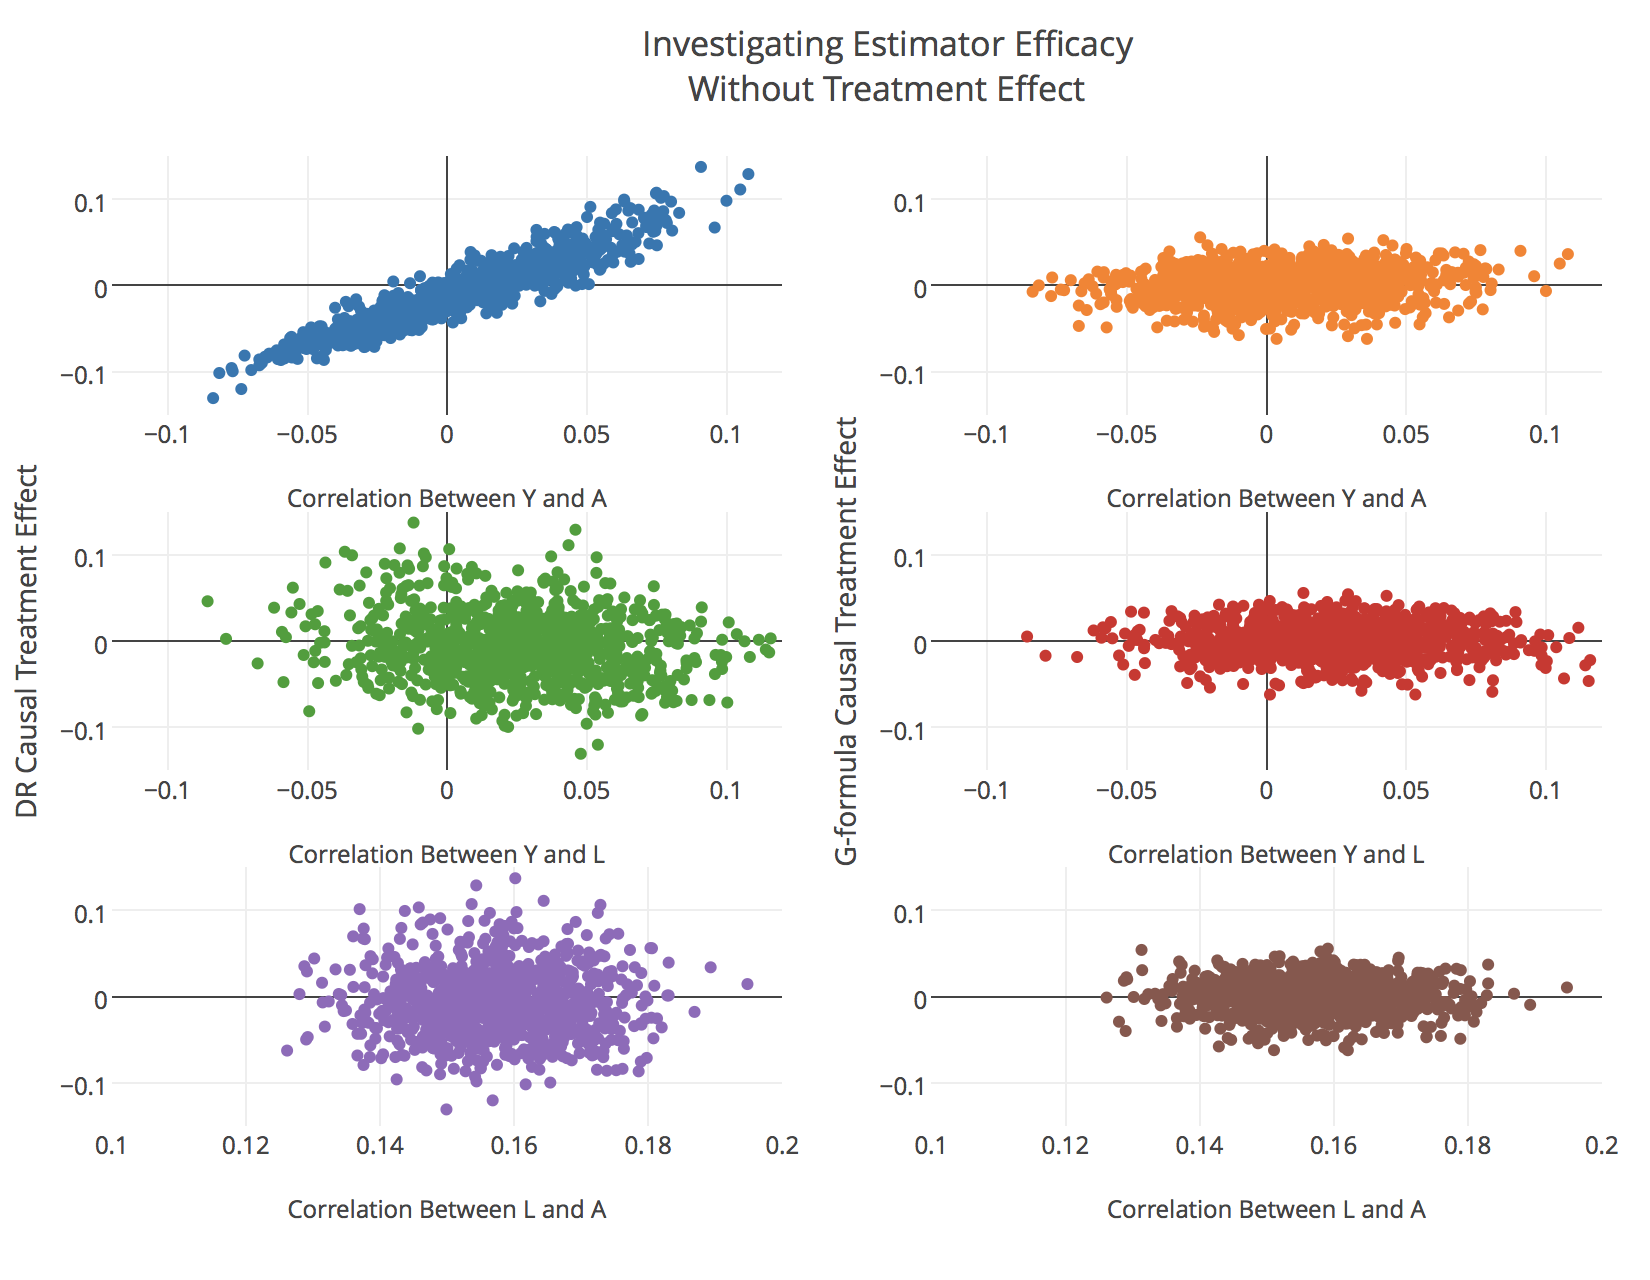
\includegraphics[width = \linewidth]{figures/correlation.png}
\caption[Scatterplots of relationships between estimates and data correlations under the null hypothesis]{Various plots showing the relationship between underlying data correlations and estimated causal treatment effects using the two methods.  Each data point is representative of one dataset.  The same 1,000 datasets are used for each effect estimation.}
\label{correlation}
\end{centering}
\end{figure}

Furthermore, the relationships between the data and the causal effect estimates were examined in Figure \ref{correlation}.  Of note, the doubly robust method is able to capture correlation between $Y$ and $A$ which the g-formula method does not, as evidenced by the first row of plots.  This is an important indicator that the doubly robust method more successfully picks up treatment effect.  This likely contributes to the more precise causal treatment effect measure.  Furthermore, the higher variance in the estimate may 


\subsection{Under the Alternative Hypothesis of Treatment} \label{alternative}
The above simulation was also tested under an alternative hypothesis of some treatment effect.  The effect was induced in the data creation algorithm by changing step \ref{datastep4} to instead be $Y_i \sim Binom(p = expit(-1+U_i + A_K + \tilde{E}(\overline{A})))$ where $\tilde{E}(\overline{A}) = \frac{1}{K} \sum_{i=1}^K A_i $ is the computational mean of the treatments throughout history.  This was in order to guarantee that $Y$ is dependent on $\overline{A}$, inducing a significant treatment effect.  

This second set of simulation testing was performed in order to determine if the methods become biased under the alternative hypothesis.  As noted in Section \ref{data}, it is not possible to directly calculate a true causal effect of $A$ on $Y$ because of the indirect dependence between $A$ and $U$.  This is at the core of why alternative methods for calculating such effects are necessary.  Because it is impossible to get an unbiased measure of the treatment effect, no biases can be calculated.  However, the results do present a few interesting findings.  Firstly, the results in Table \ref{simdata} and Figure \ref{correlation2} show that there appears to be significant issues with the g-formula under the alternative hypothesis, notably that the estimates are all zero with extreme precision and no variance.  The g-formula seems to fail to detect any treatment effect, despite the data having a definite treatment effect.  The top right graph in Figures \ref{correlation} and \ref{correlation2} show that the estimates seem to be detecting none of the correlation between $Y$ and $A$.  Considering that the method calculated quite similar, and seemingly more accurate, estimates under the alternative hypothesis as under the null, these results indicate a breakage in the g-formula method.  This is in line with the fact that under the null, the g-formula was capturing almost none of the correlation between $Y$ and $A$.  The question of what is causing this could be a mistake in the coding, a fault in the design of the models, or a violation of assumptions.
%% CONFIRM WHAT IS GOING ON HERE 

On the other hand, the doubly robust estimator appears to display a reasonable estimate for the causal effect.  It is unclear if there is any bias in this estimate since there is no calculable true causal effect estimate.  Figure \ref{correlation2} demonstrates that under the alternative, this method is again strongly capturing correlation between $Y$ and $A$.  As under the null hypothesis, the estimates seem to show low variance, indicating a low impact of randomness in the outcome.  This is another benefit of the doubly robust estimator over the g-formula, in that it does not require the incorporation of a Monte Carlo simulation which can increase variance due to randomness.  

\begin{figure}[h!]
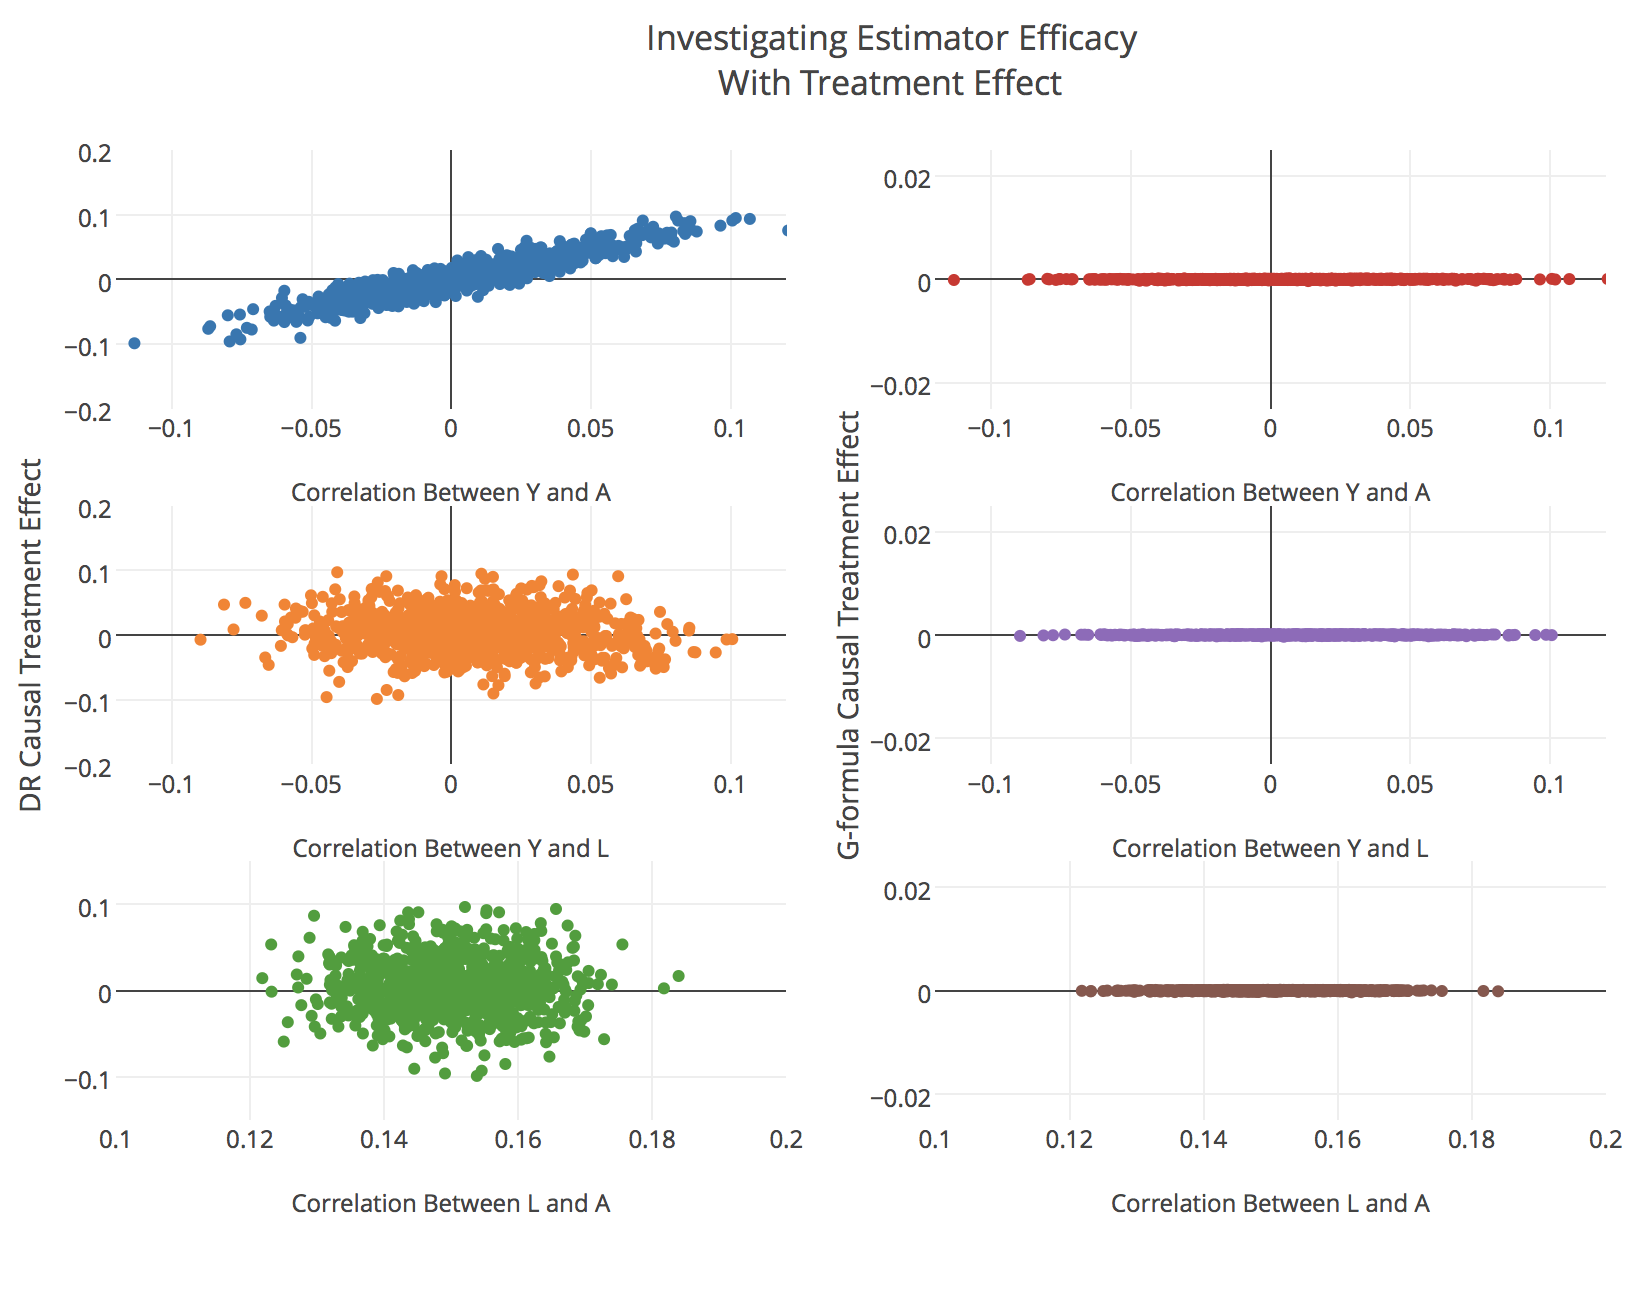
\includegraphics[width = \linewidth]{figures/correlation2.png}
\caption[Scatterplots of relationships between estimates and data correlations under the alternative hypothesis]{Various plots showing the relationship between underlying data correlations and estimated causal treatment effects using the two methods.  Each data point is representative of one dataset.  The same 1,000 datasets are used for each effect estimation.}
\label{correlation2}
\end{figure}


\newpage
\subsection{Run Times} 
In order to test the true efficiency of running these methods, run times were calculated across the 1000 simulations under both the null and alternative hypotheses.  It has traditionally been the belief that the g-formula is less efficient than the doubly robust estimator because of the Monte Carlo simulation.  However, this new implementation of it in Python was through parallelization, and as a result, it is significantly faster.  Table \ref{runtimes} shows that it takes an average of 0.38 seconds to get a g-formula estimator compared to 2.03 seconds for the doubly robust estimator.  

\begin{table}[h!]
\centering
\begin{tabular}{c | c c }
Method & Total Run Time & Average Run Time\\
\hline 
Data Generating Algorithm & 2 min, 15 sec & 0.14 sec\\ \\ 
& \multicolumn{2}{c}{\underline{Under the Null Hypothesis}} \\
G-Formula & 6 min, 19 sec & 0.38 sec \\ \\ 
Doubly Robust & 33 min, 50 sec & 2.03 sec\\ \\ 
& \multicolumn{2}{c}{\underline{Under the Alternative Hypothesis}} \\
G-Formula & 6 min, 27 sec & 0.39 sec\\ \\ 
Doubly Robust & 34 min, 5 sec & 2.05 sec
\end{tabular} \\
\centering
\caption[Run times of simulations]{This table shows the run times of the two methods implemented in Python, as well as the data generating algorithm. \label{runtimes}}
\end{table}


\section{Confirming Double Robustness} \label{doublerobust}
Twenty-five simulations were performed in order to test the double robustness of the ``doubly'' robust estimator.  Four different setups were tested: 
\begin{itemize} 
\item Using the correctly specified model for both user specified functions, $\hat{\mathbf{\alpha}}$ and $s_{m-1}$ 
\item Using an intentionally misspecified model for $\hat{\mathbf{\alpha}}$ while keeping the correct model for $s_{m-1}$ 
\item Using an intentionally misspecified model for $s_{m-1}$ while keeping the correct model for $\hat{\mathbf{\alpha}}$
\item Using intentionally misspecified models for both $\hat{\mathbf{\alpha}}$ and $s_{m-1}$ 
\end{itemize} 

The misspecified models used were as follows, 
\begin{align} 
&f(A_m \mid \overline{L}_m, \overline{A}_{m-1}; \hat{\mathbf{\alpha}}) = \alpha'_{0} + \alpha'_{1} \cdot L_{m-3} + \alpha'_{2} \cdot A_{m-3} \\ 
&s_{m}(\overline{L}_{m}, \overline{A}_{m};\mathbf{\beta}_{m}) = \beta'_0 + \beta'_1 A_{m} +\beta'_2 L_m  +\beta'_3 A_{m-4} +  \beta'_4 L_{m-4} 
 \end{align} 
These models were intentionally chosen because they are unlikely to be strong models for prediction based on the knowledge of how the data was created.  In practice, one would hope that the researcher using these methods would be wiser as not to use such terrible models, particularly for both models.  This testing is to demonstrate how robust the method is to misspecification, or how accessible the method is to those with less versed statistical knowledge as they may be more inclined to make minor mis-specifications in the model.  

The results of this testing are shown in Table \ref{doubletest} and this shows evidence that the method is indeed doubly robust.  This means that when one model is incorrect, but the other is correct, then the estimate should not be biased.  The average causal treatment effect across the simulations is not significantly impacted when either the $\hat{\mathbf{\alpha}}$ model or the $s_{m-1}$ model is incorrectly specified.  When both models are misspecified, statistically significant bias is introduced (p-value 0.005).  Furthermore, both Table \ref{doubletest} and Figure \ref{boxplot} show that the variance is significantly higher when both models are misspecified.  From the boxplot, it can be seen that the variance stays quite consistent when only one model is misspecified but is much larger when both are misspecified.  


\begin{table}[h!]
\centering
\begin{tabular} {c | c  c c}
Models & \shortstack{Average Bias in Causal \\ Treatment Effect} & p-value & \shortstack{Standard Error\\ of Bias} \\ 
\hline  \\
Both models correctly specified &0.027 & NA  & 0.0039\\ \\
$\hat{\mathbf{\alpha}}$ correct, $s_{m-1}$ misspecified & 0.030 & 0.579 & 0.0041\\ \\
$s_{m-1}$ correct, $\hat{\mathbf{\alpha}}$ misspecified& 0.030 & 0.521 &0.0042 \\ \\
Both models misspecified & 0.133 & 0.005 & 0.0355 
\end{tabular} \\
\centering
\caption[Testing double robustness]{Table showing the results of testing the double robustness of the model.  The p-value is from a two-sample t-test comparing the bias from misspecified versions with the bias results from having both models correctly specified. \label{doubletest}}
\end{table}

\begin{figure}[h!] 
\begin{centering}
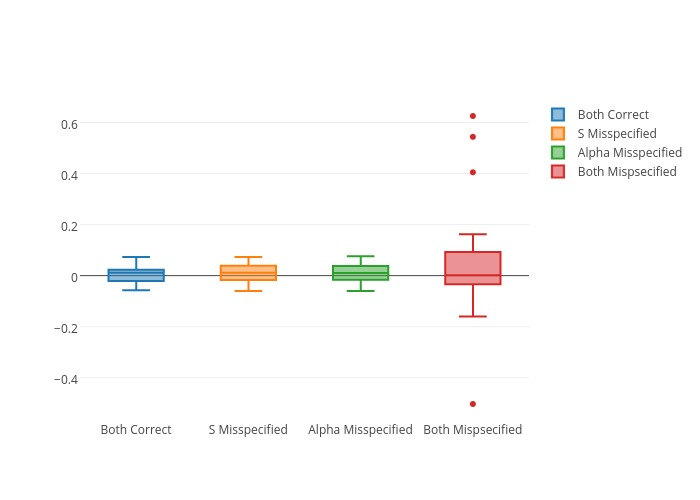
\includegraphics[width = .9\linewidth]{figures/boxplot.jpg}
\caption[Boxplot of test of double robustness]{This boxplot shows the bias in the causal treatment effect estimates for varying combinations of models correctly specified.  The fourth box, when both models are misspecified, shows the strongest bias and the most variance in that bias.  However, the model remains robust when only one model is misspecified.}
\label{boxplot}
\end{centering}
\end{figure}


\newpage
\section{Testing Multiple Robustness} \label{multiplerobust}
Having established that the model was indeed doubly robust, the model was then tested to see if it was multiply robust.  Several different combinations of correctly specified models were tested, namely of the form where the below specified models were correct and the models not listed were incorrect.  
\begin{align} 
& \pi_3, \dots, \pi_{j-1}, s_j, \dots, s_K \text{ for } j \in \{3, \dots, 12 \} \\
& s_3, \dots, s_{j-1}, \pi_j, \dots, \pi_K\text{ for } j \in \{3, \dots, 12 \}   \\
& s_3, \pi_4, s_5, \pi_6, s_7, \pi_8, s_9, \pi_{10}, s_{11}\\
& \pi_3, s_4, \pi_5, s_6, \pi_7, s_8, \pi_9, s_{10}, \pi_{11}
\end{align} 

Twenty-five simulations were performed, for which the causal treatment effect was estimated for each of these varying combinations of correctly specified models using the doubly robust method.   Then, the bias was obtained across the twenty-five estimates.  The results in Figure \ref{multirobust} show that when the correctly specified models are of the form $s_3, \dots, s_{j-1}, \pi_j, \dots, \pi_K$ for $\forall j \in \{4, \dots, 12 \} $, significant bias is introduced.\footnote{More specific values for the bias across all these models can be seen in Table \ref{MultipleTable} in Appendix \ref{AppendixB}.}  However, no bias is introduced when the correctly specified models are of the form $\pi_3, \dots, \pi_{j-1}, s_j, \dots, s_K $ for  $\forall j \in \{4, \dots, 12 \}$.  This implies that the doubly robust method is actually more robust than just doubly.  A Tukey test was also performed to test this, and the results are shown in Figure \ref{Tukey}.  The statistically significantly biased model combinations confirm the above observations.  

\begin{figure}[h!]
\centering
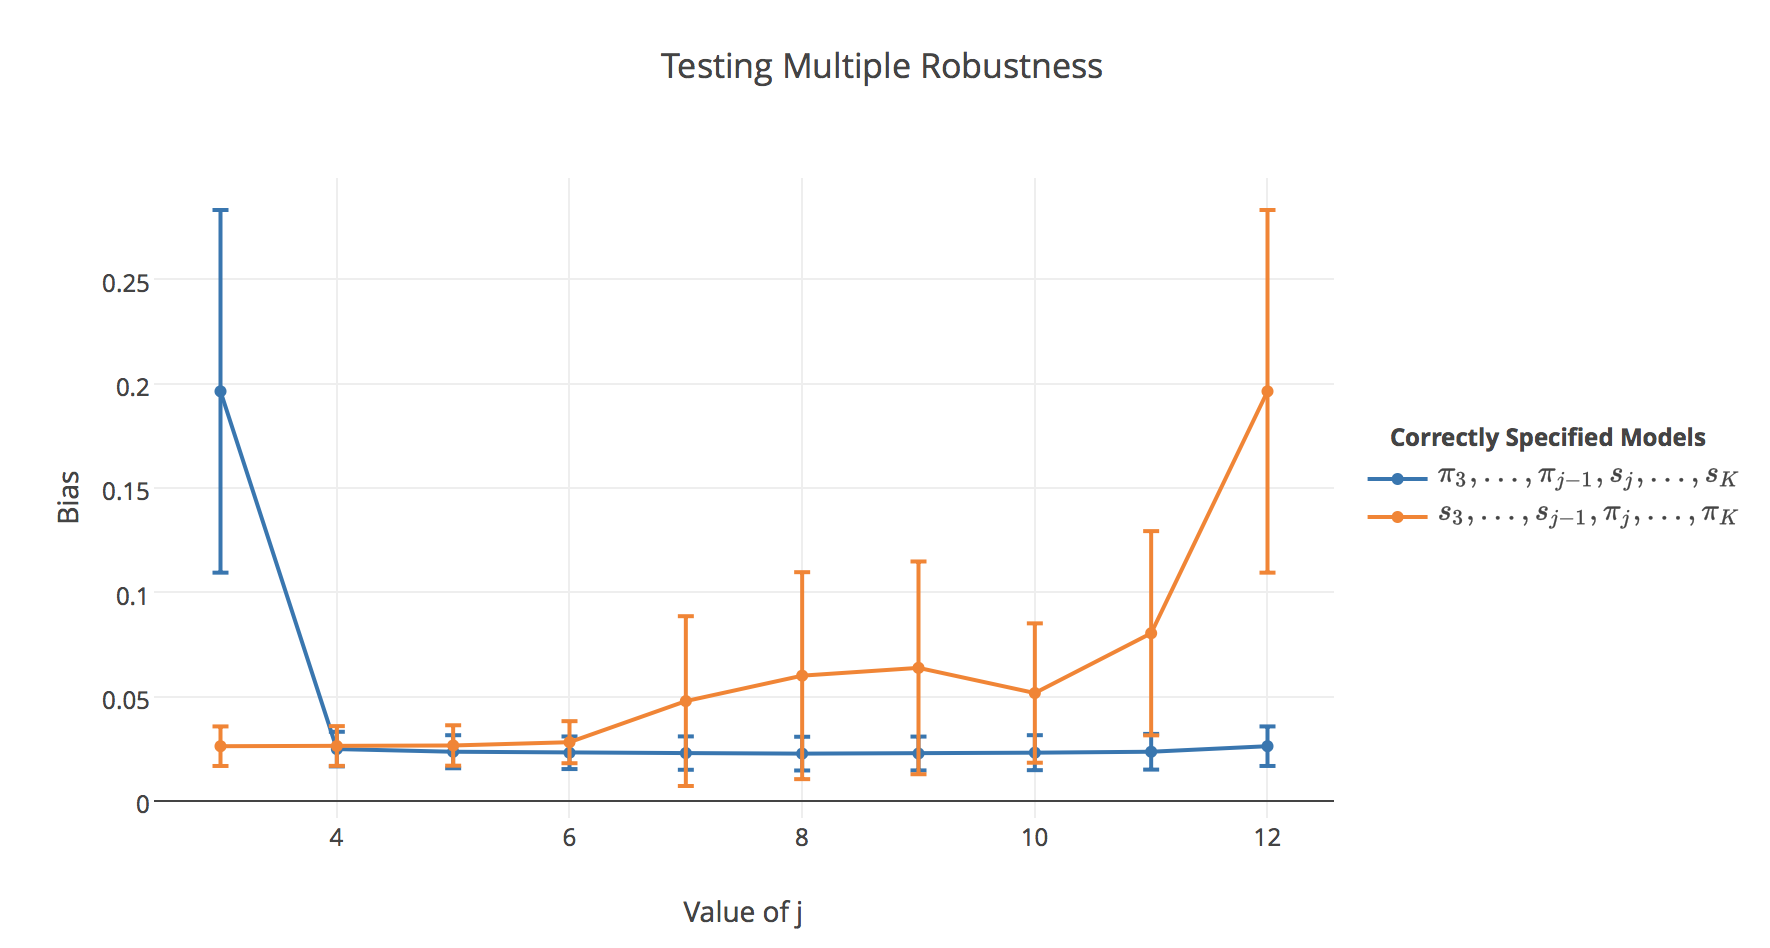
\includegraphics[width = .95\linewidth]{figures/multiplerobust.png}
\caption[Testing multiple robustness]{Plot showing the results of testing for multi-robustness.  The models are correctly specified as given in the legend.  Note that the end points of $j=3$ and $j=12$ correspond to the opposite end for the other line and represent the model where only one of the two models is correctly specified throughout.}
\label{multirobust}

\centering
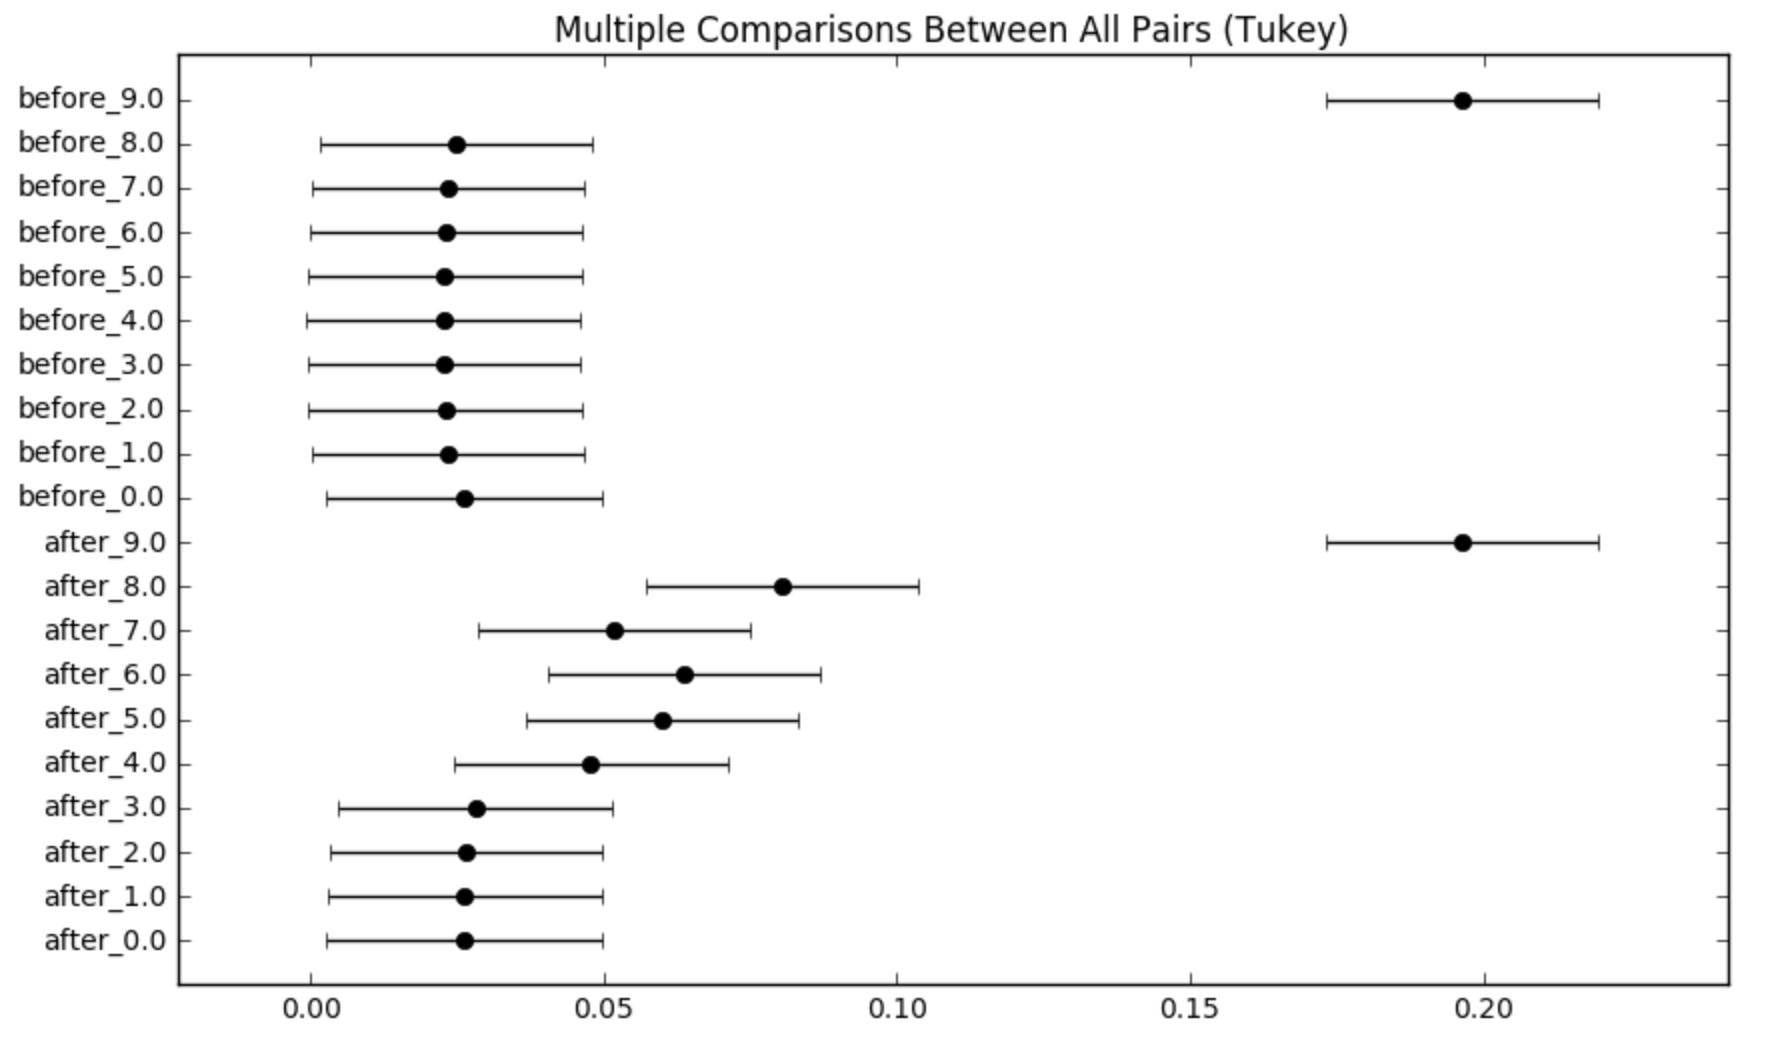
\includegraphics[width = .8\linewidth]{figures/Tukey.png}
\caption[Tukey test of multiple robustness]{A plot of the confidence intervals of each of the model specifications in the testing of multiple robustness.  The y-axis indicates which model, where the number is the value of $j$ in the following models, the before model is $\pi_3,\dots, \pi_{j-1},s_j,...,s_K$ and the after model is $s_3, \dots, s_{j-1}, \pi_j, \dots, \pi_K$.  The before and after notation signifies whether the $\pi$ models are correctly specified in order before or after the $s_m$ models.  The before values correspond to the blue lines in Figure \ref{multirobust} while the after values correspond to the orange line.}
\label{Tukey}
\end{figure} 




